% ===================== MAST-Data =====================
\subsection{MAST-Data (MAD)}\label{ds:mast_data}
\badgerow{\naturalbadge\ \okbadge\ \lbl{failure modes (trace-level)}\ \lbl{MAS, 7 frameworks}\ \lbl{8 benchmarks}}

\begin{identity}
Paper & \emph{Why Do Multi-Agent LLM Systems Fail?} --- Cemri et al. (UC Berkeley), NeurIPS 2025, arXiv:2503.13657 \cite{cemri2025mast}; introduces the MAST taxonomy and the MAD trace corpus (HF name MAST-Data)\\
Links & \href{https://huggingface.co/datasets/mcemri/MAST-Data}{HF \code{mcemri/MAST-Data}} \textperiodcentered\ \href{https://github.com/multi-agent-systems-failure-taxonomy/MAST}{GitHub \code{multi-agent-systems-failure-taxonomy/MAST}} (taxonomy, LLM annotator, notebooks)\\
License & dataset CC BY 4.0 (HF card); paper CC BY-NC-ND 4.0\\
Status & downloaded in full, ungated; \code{MAD\_full\_dataset.json} (190 MB, 1,642 traces) + \code{MAD\_human\_labelled\_dataset.json} (2.9 MB, 19 traces); \code{data/mast\_data/}. No separate \code{MAST-Data-human} repo exists\\
\end{identity}

\begin{multicols}{2}
\paragraph{Description} MAST is a grounded-theory \emph{taxonomy} of why LLM multi-agent systems fail; MAD is the companion corpus, each trace labelled with a binary vector over the 14 modes (does the mode occur anywhere in the trace?). It is a failure-mode dataset, not an attribution one: there is no faulty step, no faulty agent, no reason text and no task-outcome label. Traces are ordinary (natural) runs of 7 frameworks---AG2 (MathChat / captain-agent group chats), MetaGPT, ChatDev, Magentic-One, AppWorld, HyperAgent, OpenManus---with 5 LLMs (GPT-4o, Claude 3.7 Sonnet, GPT-4o-mini, Qwen-2.5-Coder-32B, CodeLlama-7B) on 8 benchmarks (ProgramDev, ProgramDev-v2, GSM-Plus, OlympiadBench, GAIA, MMLU, AppWorld Test-C, SWE-bench Lite). \textbf{Annotation}: (1) taxonomy built by 6 experts open-coding 150+ traces ($>$20\,h each) with three inter-annotator rounds (18 $\to$ 17 $\to$ 17 $\to$ 14 modes); (2) a human-labelled set, 3 annotators, Cohen's $\kappa$ 0.88, plus an out-of-domain round (OpenManus, Magentic-One) with $\kappa$ 0.79---21 traces in the paper, 19 in the file; (3) the full 1,642 traces labelled by an \textbf{LLM judge} (o1, few-shot) validated against the humans: accuracy 0.94, F1 0.80, $\kappa$ 0.77. The modes, with the paper's share of all failures (human study) and the number of corpus traces flagged by the judge:

\begin{center}\small
\begin{tabular}{@{}llrr@{}}\toprule
 & mode & paper \% & traces\\\midrule
\multicolumn{4}{@{}l}{\textbf{FC1 Specification issues} ($\approx$44\%)}\\
1.1 & Disobey task specification & 11.8 & 591\\
1.2 & Disobey role specification & 1.5 & 91\\
1.3 & Step repetition & 15.7 & 664\\
1.4 & Loss of conversation history & 2.8 & 117\\
1.5 & Unaware of termination conditions & 12.4 & 436\\
\multicolumn{4}{@{}l}{\textbf{FC2 Inter-agent misalignment} ($\approx$32\%)}\\
2.1 & Conversation reset & 2.2 & 80\\
2.2 & Fail to ask for clarification & 6.8 & 265\\
2.3 & Task derailment & 7.4 & 353\\
2.4 & Information withholding & 0.85 & 24\\
2.5 & Ignored other agent's input & 1.9 & 370\\
2.6 & Reasoning--action mismatch & 13.2 & 610\\
\multicolumn{4}{@{}l}{\textbf{FC3 Task verification} ($\approx$24\%)}\\
3.1 & Premature termination & 6.2 & 274\\
3.2 & No or incomplete verification & 8.2 & 608\\
3.3 & Incorrect verification & 9.1 & 658\\\bottomrule
\end{tabular}
\end{center}

\paragraph{Metrics and baselines} The paper is diagnostic; the implied task on MAD is 14-way multi-label trace classification, with the o1 judge as the only reported system (accuracy 0.94, precision 0.83, recall 0.77, F1 0.80, $\kappa$ 0.77 few-shot; $\kappa$ 0.58 zero-shot). Intervention studies: a role/workflow fix raises ChatDev task success by 9.4 points and an added verification step by 15.6 on ProgramDev (paper). MetaGPT shows 60--68\% fewer FC1/FC2 failures than ChatDev but 1.56$\times$ more FC3.

\paragraph{Schema} \code{MAD\_full\_dataset.json} is a list of records with \code{mas\_name}, \code{llm\_name}, \code{benchmark\_name}, \code{trace\_id} (0--1641), \code{trace} = \{\code{key} ``\code{<MAS>\_<bench>\_<LLM>}'', \code{index}, \code{trajectory}\} where \code{trajectory} is \emph{one raw log string} whose layout differs per framework (ChatDev/MetaGPT/OpenManus logs, AG2 printed message dicts, Magentic console transcript, AppWorld REPL, HyperAgent logger lines), and \code{mast\_annotation}: 14 keys \code{"1.1"}\ldots\code{"3.3"} $\to$ 1 / 0 / null. The human file has \code{round}, the same metadata and \code{annotations}: per mode, three boolean annotator votes; the mode list differs per round (18/17/17/14) so codes are not comparable across rounds.
\end{multicols}

\paragraph{Statistics} computed from the downloaded data.\par\nobreak\vspace{1pt}
\noindent\begin{minipage}[t]{0.48\linewidth}\vspace{0pt}\small
\begin{tabular}{@{}lr@{}}\toprule
traces: LLM-judge labelled / human-labelled & 1,642 / 19\\
(framework, benchmark, LLM) cells & 15\\
traces with $\ge$1 flag / none / all-null & 1,237 (75.5\%) / 401 / 4\\
flagged modes / trace: mean / median / max & 3.14 / 2 / 14\\
traces with any FC1 / FC2 / FC3 mode & 954 / 876 / 907\\
characters / trace: mean / median / max & 115.9\,k / 9.7\,k / 2.0\,M\\
steps / trace (heuristic): mean / median / max & 20.1 / 6 / 513\\
agents / trace (heuristic): mean / max & 3.9 / 7\\
faulty step / agent, task outcome & not labelled\\\bottomrule
\end{tabular}

\smallskip LLMs: GPT-4o 751, Claude 323, Qwen 200, CodeLlama 200, GPT-4o-mini 168. Benchmarks: ProgramDev-v2 400, ProgramDev 390, GSM 223, Olympiad 206, GAIA 195, MMLU 168, Test-C 30, SWE-bench Lite 30. Any-failure rate by framework: OpenManus and AppWorld 96.7\%, MetaGPT 94.9\%, ChatDev 92.4\%, HyperAgent 90.0\%, Magentic 78.5\%, AG2 47.9\%. Median steps: AG2 4, MetaGPT 6, Magentic 19, OpenManus 23, HyperAgent 50.5, ChatDev 66; 334 traces exceed 200\,k characters. Most common label combinations after ``none'': 1.3+1.5 (54), 1.1 alone (46), 3.2 alone (34).
\end{minipage}\hfill
\begin{minipage}[t]{0.50\linewidth}\vspace{0pt}
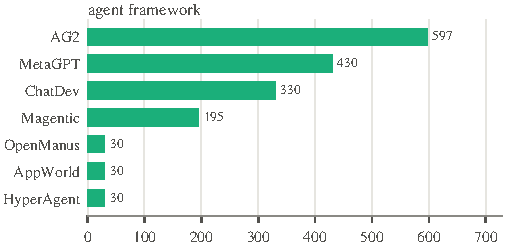
\includegraphics[width=\linewidth]{assets/figures/fw_mast_data.pdf}
\end{minipage}

\paragraph{Example trajectory} AG2 \code{trace\_id} 124 (MathChat \code{mathproxyagent} $\leftrightarrow$ \code{assistant}, GSM-Plus, Claude; 6 messages, 4.8\,k characters), flagged with FM-2.6 only. The dataset has no step label, so no step is marked: the mismatch is visible at step 1, where the assistant's code prints \$302 but its text states \$254, after which it silently switches to \$302. Steps were obtained by parsing the printed AG2 message list.
% auto-generated by scripts/render_traj.py -- do not edit
\trajtask{AG2\_GSM\_Plus\_Claude\#124 (trace\_id=\allowbreak{}124)}{Let's use Python to solve a math problem.\par Query requirements:\allowbreak{}\newline You should always use the 'print' function for the output and use fractions/\allowbreak{}radical forms instead of decimals.\newline You can use packages like sympy to help you.\newline You must follow the formats below to write your code:\allowbreak{}\newline ```python\newline \# your code\newline ```\par First state the key idea to solve the problem. You may choose from three ways to solve the problem:\allowbreak{}\newline Case 1:\allowbreak{} If the problem can be solved with Python code directly,\allowbreak{} please write a program to solve it. You\newline [...] (700 chars omitted) [...]\newline n. Spaying her cost \$200,\allowbreak{} her 3 vaccines cost \$20 each,\allowbreak{} but Leah got a 10\% discount on the total vaccine cost,\allowbreak{} and the kitten broke 4 vases that cost \$12 each. How much has the kitten cost so far?\allowbreak{}}
\begin{trajstep}{0}{mathproxyagent}{agA}
Let's use Python to solve a math problem.\par Query requirements:\allowbreak{}\newline You should always use the 'print' function for the output and use fractions/\allowbreak{}radical forms instead of decimals.\newline You can use packages like sympy to help you.\newline You must follow the formats below to write your code:\allowbreak{}\newline ```python\newline \# your code\newline ```\par First state the key idea to solve the problem. You may choose from three ways to solve the problem:\allowbreak{}\newline Case 1:\allowbreak{} If the problem can be solved with Python code directly,\allowbreak{} please write a program to solve it. You can enumerate all possible arrangements if needed.\newline Case 2:\allowbreak{} If the problem is mostly reasoning,\allowbreak{} you can solve it by yourself directly.\newline Case 3:\allowbreak{} If\newline [...] (500 chars omitted) [...]\newline answer in \textbackslash{}boxed\{\}.\par Problem:\allowbreak{}\newline Leah just got a new kitten. Spaying her cost \$200,\allowbreak{} her 3 vaccines cost \$20 each,\allowbreak{} but Leah got a 10\% discount on the total vaccine cost,\allowbreak{} and the kitten broke 4 vases that cost \$12 each. How much has the kitten cost so far?\allowbreak{}
\end{trajstep}
\begin{trajstep}{1}{assistant}{agB}
\# Key Idea\newline I'll solve this problem directly with Python code. We need to calculate the total cost which includes:\allowbreak{}\newline 1. Spaying cost:\allowbreak{} \$200\newline 2. Vaccines cost:\allowbreak{} 3 vaccines at \$20 each with a 10\% discount\newline 3. Broken vases:\allowbreak{} 4 vases at \$12 each\par ```python\newline from fractions import Fraction\par \# Calculate the costs\newline spaying\_cost =\allowbreak{} 200\newline vaccine\_cost\_per\_unit =\allowbreak{} 20\newline number\_of\_vaccines =\allowbreak{} 3\newline vaccine\_discount =\allowbreak{} Fraction(10,\allowbreak{} 100) \# 10\%\newline vaccine\_cost =\allowbreak{} number\_of\_vaccines * vaccine\_cost\_per\_unit * (1 - vaccine\_discount)\par vase\_cost\_per\_unit =\allowbreak{} 12\newline number\_of\_vases =\allowbreak{} 4\newline vase\_cost =\allowbreak{} number\_of\_vases * vase\_cost\_per\_unit\par total\_cost =\allowbreak{} spaying\_cost + vaccine\_cost + vase\_cost\par print(f"Spaying cost:\allowbreak{} \$\{spaying\_cost\}")\newline print(f"Vaccine cost (with discount):\allowbreak{} \$\{vaccine\_cost\}")\newline print(f"Cost of broken vases:\allowbreak{} \$\{vase\_cost\}")\newline print(f"Total cost:\allowbreak{} \$\{total\_cost\}")\newline ```\par The answer is \textbackslash{}boxed\{\$254\}.
\end{trajstep}
\begin{trajstep}{2}{mathproxyagent}{agA}
Spaying cost:\allowbreak{} \$200\newline Vaccine cost (with discount):\allowbreak{} \$54\newline Cost of broken vases:\allowbreak{} \$48\newline Total cost:\allowbreak{} \$302
\end{trajstep}
\begin{trajstep}{3}{assistant}{agB}
I need to review my calculations as the output shows a discrepancy. Let me recalculate:\allowbreak{}\par \# Key Idea\newline I'll solve this problem directly with Python code but with corrected calculations. Let me carefully check each part:\allowbreak{}\par ```python\newline from fractions import Fraction\par \# Calculate the costs\newline spaying\_cost =\allowbreak{} 200\par \# Vaccine calculations - 3 vaccines at \$20 each,\allowbreak{} then 10\% discount on the total\newline vaccine\_cost\_per\_unit =\allowbreak{} 20\newline number\_of\_vaccines =\allowbreak{} 3\newline vaccine\_subtotal =\allowbreak{} number\_of\_vaccines * vaccine\_cost\_per\_unit\newline vaccine\_discount =\allowbreak{} Fraction(10,\allowbreak{} 100) \# 10\%\newline vaccine\_cost =\allowbreak{} vaccine\_subtotal * (1 - vaccine\_discount)\par \# Broken vases - 4 vases at \$12 each\newline vase\_cost\_per\_u\newline [...] (399 chars omitted) [...]\newline ion. Let me correct the analysis manually:\allowbreak{}\par 1. Spaying cost:\allowbreak{} \$200\newline 2. Vaccines:\allowbreak{} 3 vaccines at \$20 each =\allowbreak{} \$60,\allowbreak{} with 10\% discount =\allowbreak{} \$60 - \$6 =\allowbreak{} \$54\newline 3. Broken vases:\allowbreak{} 4 vases at \$12 each =\allowbreak{} \$48\par Total cost:\allowbreak{} \$200 + \$54 + \$48 =\allowbreak{} \$302\par The answer is \textbackslash{}boxed\{\$302\}.
\end{trajstep}
\begin{trajstep}{4}{mathproxyagent}{agA}
Spaying cost:\allowbreak{} \$200\newline Vaccine subtotal:\allowbreak{} \$60\newline Vaccine cost (with discount):\allowbreak{} \$54\newline Cost of broken vases:\allowbreak{} \$48\newline Total cost:\allowbreak{} \$302
\end{trajstep}
\begin{trajstep}{5}{assistant}{agB}
Great! The calculations are now correct.\par \# Final Solution\newline Let's summarize the costs:\allowbreak{}\par 1. Spaying cost:\allowbreak{} \$200\newline 2. Vaccines:\allowbreak{} 3 vaccines at \$20 each =\allowbreak{} \$60 subtotal,\allowbreak{} with 10\% discount =\allowbreak{} \$54\newline 3. Broken vases:\allowbreak{} 4 vases at \$12 each =\allowbreak{} \$48\par Adding all these up:\allowbreak{} \$200 + \$54 + \$48 =\allowbreak{} \$302\par The answer is \textbackslash{}boxed\{\$302\}
\end{trajstep}
\trajannotation{—}{---}{["FM-2.6 Reasoning-action mismatch (FC2 Inter-agent misalignment)"]}{}{—}{Great! The calculations are now correct.\par \# Final Solution\newline Let's summarize the costs:\allowbreak{}\par 1. Spaying cost:\allowbreak{} \$200\newline 2. Vaccines:\allowbreak{} 3 vaccines at \$20 each =\allowbreak{} \$60 subtotal,\allowbreak{} with 10\% discount =\allowbreak{} \$54\newline 3.\newline [...] (41 chars omitted) [...]\newline Adding all these up:\allowbreak{} \$200 + \$54 + \$48 =\allowbreak{} \$302\par The answer is \textbackslash{}boxed\{\$302\}}{\textbf{mast\_annotation}: \{"1.1":\allowbreak{} 0,\allowbreak{} "1.2":\allowbreak{} 0,\allowbreak{} "1.3":\allowbreak{} 0,\allowbreak{} "1.4":\allowbreak{} 0,\allowbreak{} "1.5":\allowbreak{} 0,\allowbreak{} "2.1":\allowbreak{} 0,\allowbreak{} "2.2":\allowbreak{} 0,\allowbreak{} "2.3":\allowbreak{} 0,\allowbreak{} "2.4":\allowbreak{} 0,\allowbreak{} "2.5":\allowbreak{} 0,\allowbreak{} "2.6":\allowbreak{} 1,\allowbreak{} "3.1":\allowbreak{} 0,\allowbreak{} "3.2":\allowbreak{} 0,\allowbreak{} "3.3":\allowbreak{} 0\}; \textbf{mas\_name}: AG2; \textbf{llm\_name}: Claude; \textbf{benchmark\_name}: GSM; \textbf{annotator}: LLM judge (OpenAI o1,\allowbreak{} few-shot) --- trace-level binary labels only; \textbf{step\_split}: heuristic:\allowbreak{} AG2 message list parsed with ast.literal\_eval;\allowbreak{} agent =\allowbreak{} message `name`}


\paragraph{Notes} (i) Taxonomy corpus, not attribution benchmark: trace-level binary flags only---usable for mode classification and taxonomy statistics, not for localisation metrics. (ii) Only 19 traces carry human labels; the corpus labels are o1's ($\kappa$ 0.77), and corpus shares differ from the paper's human frequencies, notably FM-2.5 (7.2\% of flags vs.\ 1.9\%) and FM-3.2/3.3. Our per-round $\kappa$ on the human file is 1.00 for rounds 1--2, which suggests post-discussion consolidated labels. (iii) Seven raw log layouts (1\,k--2\,M characters); any step-level use needs framework-specific parsers (ours are in \code{scripts/analyze\_mast.py}; 32 AG2/HyperAgent traces fail to parse). (iv) Framework, benchmark and LLM are confounded: most cells pair one framework with one LLM (all HyperAgent runs are Claude on SWE-bench Lite). (v) Quirks: 4 all-null annotations, swapped \code{mas\_name}/\code{benchmark\_name} on the two GAIA rows of the human file, round name ``Generlazability''. (vi) Overlaps: Magentic-One/GAIA traces share task source with Who\&When, TRAIL and CORRECT-Error; SWE-bench Lite with TRAIL and AgentErrata; MAST is the reference taxonomy that AgentErrata's and several other 2025--26 datasets' modes map onto.
